\section{Lecture 26}
\subsection{Lecture Notes - Liouville's Theorem, Path to QM (Canonical Quantization)}
\subsubsection{Review - Liouville's Theorem}
\begin{itemize}
    \item The volume $V$ of a region of phase space does not change in time.
    \item The phase space density $N/V$ moving with the slow lines remains constant.
    \item The phase space density moves like an incompressible fluid.
    \item $V_t = \int d\v{z}_t = \int\abs{\dpd{\v{z}_t}{\v{z}_0}}d\v{z}_0 = V_0$, $abs{\dpd{\v{z}_t}{\v{z}_0}} = 1$
\end{itemize}

\subsubsection{Liouville's Theorem from Gauss's (Divergence) Theorem}
Recall the divergence theorem; for a vector field $\v{v}$, it holds that:
\[\int_V \div{\v{v}} dV = \int_S \v{v} \cdot \v{n} dA\]
Now we consider the divergence of the phase space velocity, $\v{v}$:
\[\v{v} = \m{\dot{\v{q}} \\ \dot{\v{p}}} = \m{\dpd{\HH}{\v{p}} \\ -\dpd{\HH}{\v{q}}}\]
The divergence is given by:
\[\div{\v{v}} = \dpd{\dot{\v{q}}}{\v{q}} + \dpd{\dot{\v{p}}}{\v{p}} = \dpd{}{\v{q}}\left(\dpd{\HH}{\v{p}}\right) - \dpd{}{\v{p}}\left(\dpd{\HH}{\v{q}}\right) = 0\]
Where we use Hamilton's equations and the equality of mixed partials. How do we interpret this? Consider a surface in phase space that moves out with time. As the surface expands there will be a change in volume covered by this propagating surface.
\begin{center}
    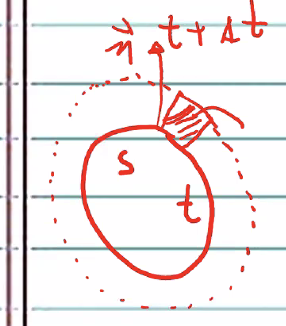
\includegraphics[scale=0.7]{Lecture-26/l26-img1.png}
\end{center}
Giving this a surface normal $\v{n}$, calculating the change in volume w.r.t. time we have $\delta V = \v{n}\cdot \v{v}\delta t dA$ and if we integrate over the entire surface, we get teh total change. This yields $\Delta V = \int_S \v{n} \cdot \v{v}\Delta t dA$. And hence:
\[\dod{V}{t} = \int_S \v{n}\cdot \v{v}dA = 0\]
Where the RHS we set to zero by the divergence theorem. This concludes the proof, and is another way of proving the theorem.

\subsubsection{Poisson Brackets Revisited \& The path to QM}
Recall we could write:
\[\dod{F}{t} = [F, \HH] + \dpd{F}{t}\]
where $F$ is some function on phase space. By definition, we had:
\[[F, G] = \sum_i \dpd{F}{q_i}\dpd{G}{p_i} - \dpd{F}{p_i}\dpd{G}{q_i}\]
The fundamental poisson brackets of position and momentum were given by:
\[[q_i, q_j] = [p_i, p_j] = 0, \quad [q_i, p_j] = \delta_{ij}\]
We now connect this to QM, one of the defining theories of the 20th century. 

\noindent Recall that in QM, measurements are operations. We perturb systems by measuring/observing them (e.g. measure position of ball by shining light on it, but light carries momentum, so it will interact with the ball in doing so.). Also recall that in qm, $pq$ and $qm$ are different, that is that operators do not (in general) commute. 

\subsubsection{Non-Commutative Structure of Phase Space}
Phase space functions become non-commutative operators (matrices).
\noindent Consider four phase space functions, $F_1, F_2, G_1, G_2$. Now, consider the object $[F_1F_2, G_1G_2]$. We pull this apart using the Leibniz product rule:
\[[F_1F_2, G_1G_2] = [F_1, G_1G_2]F_2 + F_1[F_2, G_1G_2] \]
we can also apply it on the second argument:
\[[F_1F_2, G_1G_2] = [F_1F_2, G_1]G_2 + G_1[F_1F_2, G_2]\]
Hence, we get the following expression if we apply hte product rule again:
\[[F_1F_2, G_1G_2] = [F_1, G_1](F_2G_2 - G_2F_2) = (F_1G_1 - G_1F_1)[F_2, G_2]\]
If we have classical observables, the $F, G$s are just numbers, they commute and the relation is obviously satisfied (both sides are just zero!). But in QM, we want to consider arbitrary, non-commuting operators. Hence, the condition for the above equation to be satified for arbitrary non-commuting operators is that:
\[[F_1, G_1] = F_1G_1 - G_1F_1\]
That is, we want the Poisson bracket to be a commutator. Furthermore, we will embellish this with an imaginary unit $i$:
\[i[F_1, G_1] = F_1G_1 - G_1F_1\]
Which is there to ensure that the bracket of two Hermitian operators is again Hermitian. Recall that a Hermitian operator $O$ satisfies $O^\dagger = O$. Finally, we put a number $\hbar$ in front of the commutator as well:
\[i\hbar[F_1, G_1] = F_1G_1 - G_1F_1\]
This now gives the quantum mechanics we know. This process is known as \textbf{canonical quantization}.

\subsubsection{Canonical Quantization}
There are two steps of going from classical mechanics to quantum mechanics:
\begin{enumerate}
    \item Phase space functions (numbers) turn into operators (non-commuting in general).
    \item $[F, G]_P \mapsto \frac{1}{i \hbar}[F, G]$, that is, we embellish the poisson bracket with a factor of $i\hbar$ and turn it into a commutator.
\end{enumerate}
We can check the canonical commutation relations of quantum mechanics:
\[[q_i, q_j] = [p_i, p_j] = 0\]
\[[p_i, p_j] = i\hbar\delta_{ij}\]
From these relations, we can derive many fundamental results of quantum mechanics, such as the Heisenberg uncertainty principle, that is, $(\Delta q)(\Delta p) \geq \frac{\hbar}{2}$. By making the Poisson bracket the commutator, we get this quantized theory with uncertainty built into it. We may also look at the time evolution of operators. The classical evolution equation is:
\[\dod{F}{t} = [F, H]_P + \dpd{F}{t}\]
the quantum version of this replaces the poisson bracket with a commutator; for a quantum mechanical operator $O$, the time evolution of it is given by:
\[\boxed{\dod{O}{t} = -\frac{i}{\hbar}[O, H] + \dpd{O}{t}}\]
Which is known as the Heisenberg equation of motion. This is the Heisenberg picture of QM, where you move the idea of time-evolution from the states (the Schrodinger picture) to the operators. The canonical quantization process takes us into the Heisenberg picture. Note that one can also do this on fields and get Quantum Field Theory, but that is a story for another course.